\documentclass{ctexart}
\usepackage{xcolor}
\usepackage{setspace}
\usepackage{tikz}
\usepackage{ctex}
\usepackage{geometry}
\usepackage{amsmath}
\usepackage{graphicx} 
\usepackage{subfigure}
\usepackage{float}
\usepackage{algorithm}  
\usepackage{algorithmicx}  
\usepackage{algpseudocode} 
\usepackage{url}
\usepackage{amsthm, amssymb, appendix, bm, graphicx, hyperref, mathrsfs}
\usepackage{tabularx}
\usepackage{booktabs} %需要加载宏包{booktabs}
\usepackage{multirow}
\usepackage{diagbox} % 加载宏包
\usepackage{pifont}

\usepackage{siunitx}
\usepackage{listings}
\usepackage{float}
\pagestyle{plain}

\usetikzlibrary{datavisualization}
\usetikzlibrary{arrows,shapes,chains}
\usepackage{listings}
\lstset{language=C++}
\lstset{breaklines}
\lstset{extendedchars=false}
\lstset{numbers=left}
\geometry{a4paper,left=2.5cm,right=2.5cm,top=2.5cm,bottom=2.5cm}
\CTEXsetup[format={\Large\bfseries\centering}]{section}
\tikzstyle{startstop} = [rectangle,rounded corners, minimum width=3cm,minimum height=1cm,text centered, text width=6cm,draw=black]
\tikzstyle{io} = [trapezium, trapezium left angle = 70,trapezium right angle=110,minimum width=5cm,minimum height=1cm,text centered,draw=black,fill=white]
\tikzstyle{process} = [rectangle,minimum width=3cm,minimum height=1cm,text centered,text width =3cm,text width=6cm,draw=black]
\tikzstyle{decision} = [diamond,minimum width=3cm,minimum height=1cm,text centered,text width=6cm,aspect=2,draw=black,thin]
\tikzstyle{arrow} = [thick,->,>=stealth]
\renewcommand{\algorithmicrequire}{\textbf{Input:}}  % Use Input in the format of Algorithm  
\renewcommand{\algorithmicensure}{\textbf{Output:}} % Use Output in the format of Algorithm  
\newcommand{\subsubsubsection}[1]{\paragraph{#1}\mbox{}\\}
\setcounter{secnumdepth}{4} % how many sectioning levels to assign numbers to
\setcounter{tocdepth}{4} % how many sectioning levels to show in ToC
\begin{document}

\section{模型假设}
1. \quad 基于自身感知的高度信息,本文默认无人机均保持在同一个高度上飞行,即所有无人机在同一个平面上。

2. \quad 假设第一问中的所有小问9架无人机理论上都应均匀分布在半径为100m的圆周上。

3. \quad 假设无人机接收到的方向信息不存在误差。


\subsection{问题一模型的建立与求解}

\subsubsection{极坐标系的建立}

为了更加明确地标注出各编号无人机的标准位置,我们选用包含角度信息的极坐标系来进行刻画。由于被动接收信号的无人机仅能接收到方向信息,即角度,故极坐标系相比直角坐标系更易表达清晰。

假设9架无人机(编号FY01$\sim$FY09)均匀分布在一个半径为100m的圆周上。以编号FY00的无人机作为坐标原点,编号FY00与编号FY01之间的连线作为X轴,建立极坐标系如下图。各个编号的标准坐标信息如下表:

\begin{figure}[htbp]
  \centering
  \includegraphics[width=0.40\linewidth]{pic/极坐标.jpg}
  \caption{极坐标系示意图}
  \end{figure} 

\begin{center}
  表1:各编号无人机标准坐标
  ~\\
    \begin{tabular}{|c|c|c|c|c|c|}
        \hline
        无人机编号&极坐标(m,$^{\circ}$)&无人机编号&极坐标(m,$^{\circ}$)&无人机编号&极坐标(m,$^{\circ}$)\\
        \hline
        FY00&(0,0)&FY01&(100,0)&FY02&(100,40)\\
        \hline
        FY03&(100,80)&FY04&(100,120)&FY05&(100,160)\\
        \hline
        FY06&(100,200)&FY07&(100,240)&FY08&(100,280)\\
        \hline
        FY09&(100,320)& & & &\\    

        \hline
    \end{tabular}\\
\end{center}
\subsubsection{定位模型的建立}
题目要求在已知未知定位无人机与任意两架发射源无人机间连线的夹角后,给出未知定位无人机当前的所在位置。由于发射源无人机的位置是无偏差的,故它们间的距离同样为已知信息。对该问题进行几何分析:

图中A、B、C三点为已知位置的发射源无人机(A为原点,B、C点在圆上按逆时针顺序排列),三点将平面区域划分为4各部分。D点为需要求解的无人机的位置,可能落在任意一个区域中。

其中,A、B和A、C间的距离均为半径r。已知的方向信息包含两个小角与小角组合形成的大角,实际有效信息仅含两个角度。为了方便计算,我们选择包含原点A的角度$\alpha_1$、$\alpha_2$以及发射源无人机间的夹角$\alpha_3$进行分析。

对每个部分的点分别建立定位模型如下:

利用正弦定理及角度关系对$\Delta$ABD,$\Delta$ACD,$\Delta$BCD进行分析,分别列出下列等式:

设$\angle ABD=\theta_1$,$\angle ACD=\theta_2$,$\angle ADB=\alpha_1$,$\angle ADC=\alpha_2$,$\angle BAC=\alpha_3$,AD=l。

(1)若$\alpha_1$、$\alpha_2$之间不存在包含关系,即D点落在I、III区域,分为两种情况讨论:

若D点落在I区域,如图,则:

\begin{figure}[htbp]
  \centering
  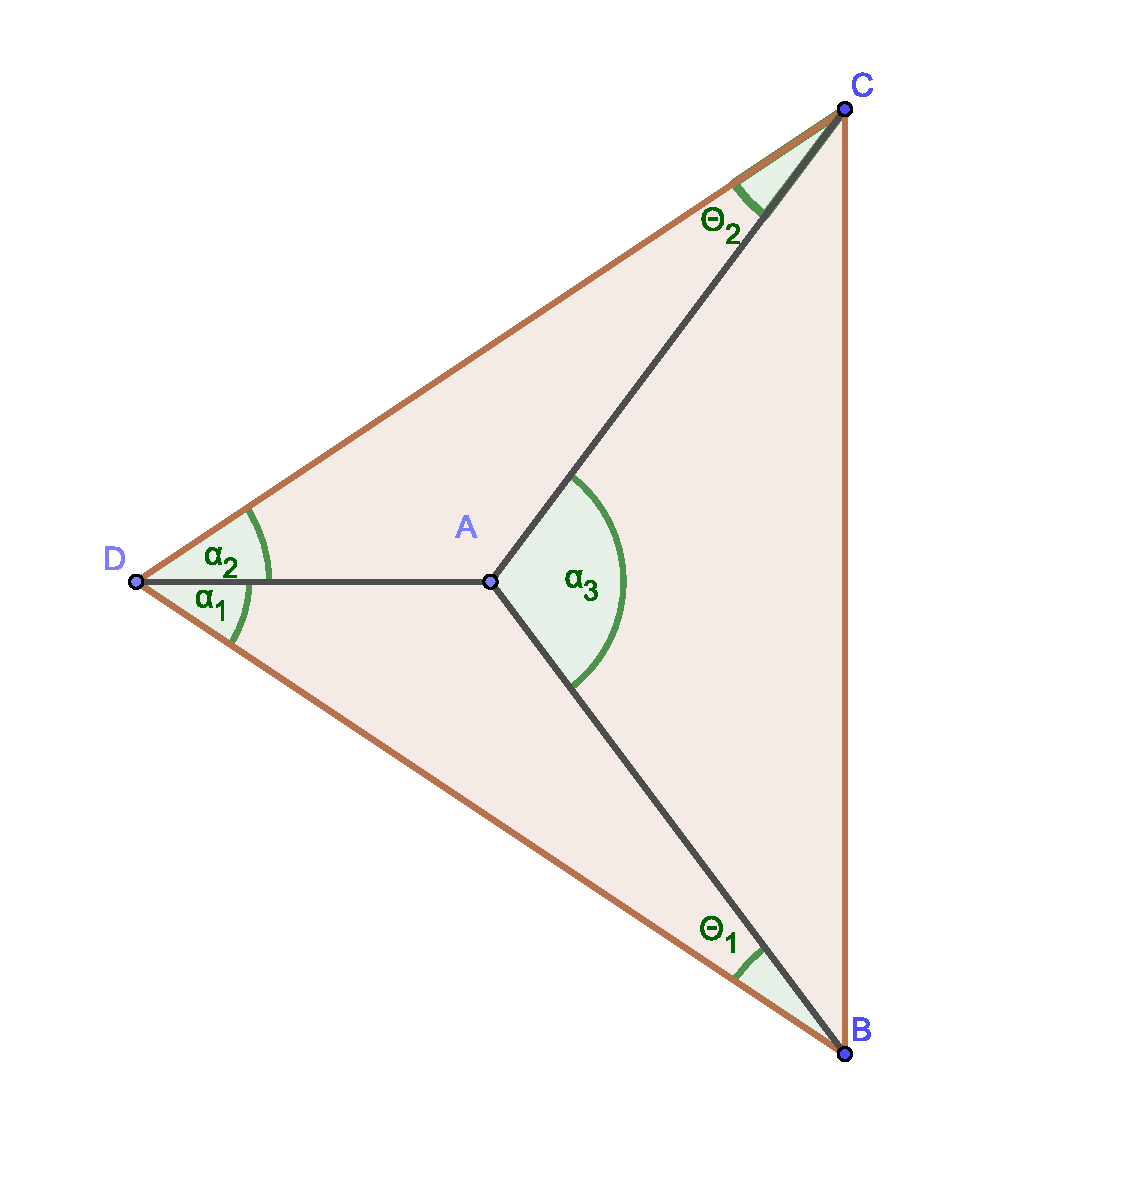
\includegraphics[width=0.40\linewidth]{pic/case1++.eps}
  \caption{区域I典型图}
  \end{figure} 

\begin{equation}
    \left\{
              \begin{array}{ll}
                \theta_1+\theta_2=\alpha_3-(\alpha_1+\alpha_2)=\theta_0\\
                \frac{sin\theta_1}{l}=\frac{sin\alpha_1}{r}=k_1\\
                \frac{sin\theta_2}{l}=\frac{sin\alpha_2}{r}=k_2\\

              \end{array}
            \right.
\end{equation}

\[
    \Rightarrow sin(\theta_0-\theta_1)=\frac{k_2}{k_1}sin\theta_1
\]
\[
    \Rightarrow sin\theta_0 \cdot cos\theta_1-cos\theta_0 \cdot sin\theta_1=\frac{k_2}{k_1}sin\theta_1
\]

\[
    \Rightarrow \theta_1=arctan(\frac{sin\theta_0}{\frac{sin\alpha_2}{sin\alpha_1}+cos\theta_0}),\theta_0=\alpha_3-(\alpha_1+\alpha_2)
\]

在求解过程中,如果发现等式无法计算或出现正无穷的情况,则考虑$\theta_1=90^{\circ}$。

若B的极坐标为(100,$\beta$),则该种情况下,未知点的定位坐标为(100$\times\frac{sin\theta_1}{sin\alpha_1}$,$\beta -$($\pi$-$\theta_1$-$\alpha_1$))。



若D点落在III区域,如图,则:

\begin{figure}[htbp]
  \centering
  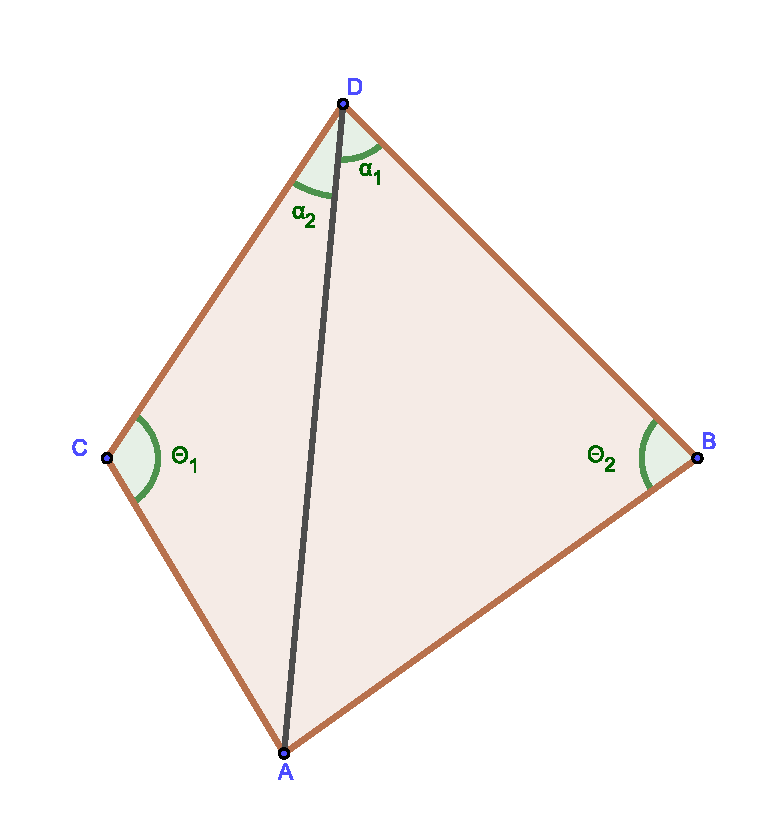
\includegraphics[width=0.40\linewidth]{pic/case3+.eps}
  \caption{区域III典型图}
  \end{figure} 


无论D点在$\Delta ABC$内部还是外部,所建立的方程保持不变。

\begin{equation}
    \left\{
              \begin{array}{ll}
                \theta_1+\theta_2=2\pi-(\alpha_1+\alpha_2+\alpha_3)\\
                \frac{sin\theta_1}{l}=\frac{sin\alpha_1}{r}=k_1\\
                \frac{sin\theta_2}{l}=\frac{sin\alpha_2}{r}=k_2\\

              \end{array}
            \right.
\end{equation}
\[
    \Rightarrow \theta_1=arctan \frac{-sin(\alpha_1+\alpha_2+\alpha_3)}{\frac{sin\alpha_2}{sin\alpha_1}+cos(\alpha_1+\alpha_2+\alpha_3)}
\]
或$\theta_1=90^{\circ}$。

若B的极坐标为(100,$\beta$),则该种情况下,未知点的定位坐标为(100$\times\frac{sin\theta_1}{sin\alpha_1}$,$\beta +$($\pi$-$\theta_1$-$\alpha_1$))。


(2)若$\alpha_1$、$\alpha_2$之间存在包含关系,即D点落在II、IV区域,两种可能性如图所示;

\begin{figure}[htbp]
  \begin{minipage}[t]{0.45\linewidth}
  \centering
  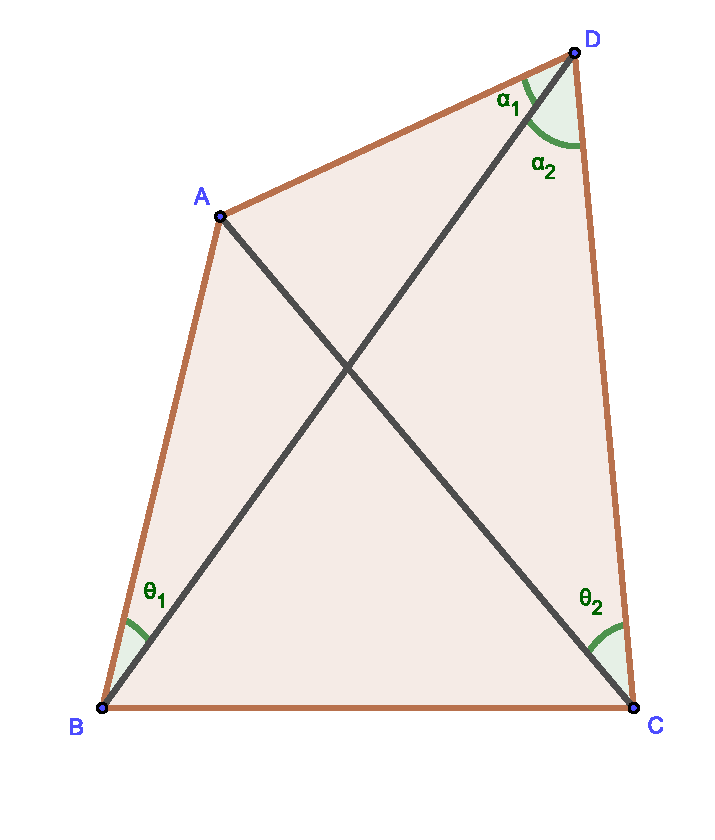
\includegraphics[height=5.5cm,width=5.5cm]{pic/case4.eps}
  \caption{区域II典型图}
  \end{minipage}%
  \begin{minipage}[t]{0.45\linewidth}
  \centering
  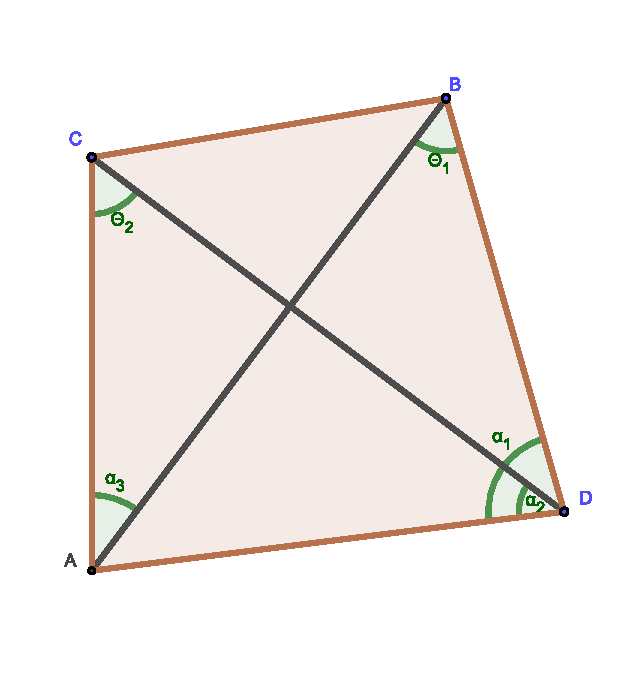
\includegraphics[height=5.5cm,width=5.5cm]{pic/case2+.eps}
  \caption{区域IV典型图}
  \end{minipage}
  \end{figure}


当$\alpha_1 < \alpha_2$时:

\begin{equation}
    \left\{
              \begin{array}{ll}
                \theta_1-\theta_2=\alpha_2-(\alpha_1+\alpha_3)=\theta_0\\
                \frac{sin\theta_1}{l}=\frac{sin\alpha_1}{r}=k_1\\
                \frac{sin\theta_2}{l}=\frac{sin\alpha_2}{r}=k_2\\

              \end{array}
            \right.
\end{equation}

\[
    \Rightarrow \theta_1=arctan\frac{sin\theta_0}{cos\theta_0-\frac{sin\alpha_2}{sin\alpha_1}},\theta_0=\alpha_2-(\alpha_1+\alpha_3)
\]
或$\theta_1=90^{\circ}$。

若B的极坐标为(100,$\beta$),则该种情况下,未知点的定位坐标为(100$\times\frac{sin\theta_1}{sin\alpha_1}$,$\beta +$($\pi$-$\theta_1$-$\alpha_1$))。


当$\alpha_1 > \alpha_2$时:

\begin{equation}
    \left\{
              \begin{array}{ll}
                \theta_2-\theta_1=\alpha_1-(\alpha_2+\alpha_3)=\theta_0\\
                \frac{sin\theta_1}{l}={sin\alpha_1}{r}=k_1\\
                \frac{sin\theta_2}{l}={sin\alpha_2}{r}=k_2\\

              \end{array}
            \right.
\end{equation}

\[
    \Rightarrow \theta_1=arctan\frac{sin\theta_0}{\frac{sin\alpha_2}{sin\alpha_1}-cos\theta_0},\theta_0=\alpha_1-(\alpha_2+\alpha_3)
\]
或$\theta_1=90^{\circ}$。

若B的极坐标为(100,$\beta$),则该种情况下,未知点的定位坐标为(100$\times\frac{sin\theta_1}{sin\alpha_1}$,$\beta -$($\pi$-$\theta_1$-$\alpha_1$))。

由于$\theta_1$有四种不同的表达方式,故未知点仍有四个可能的坐标位置。 

\subsubsubsection{最终位置的确定}

由于我们无从知道D点究竟落在哪个区域,故四个点的坐标均有可能。然而题目中提及被动接收信号无人机所在位置仅略有偏差,故我们考虑将求解出来的四个坐标分别与标准坐标求欧几里得距离,将其中距离最短的点作为该无人机所在的位置。

距离公式计算方式如下:

设D点的标准坐标为(100,$\gamma_0$),求解出来的其中一个坐标为(100$\times\frac{sin\theta_1}{sin\alpha_1}$,$\beta \pm$($\pi$-$\theta_1$-$\alpha_1$)),则:

\[
 s=\sqrt{100^2+(100\times\frac{sin\theta_1}{sin\alpha_1})^2-2\times100\times(100\times\frac{sin\theta_1}{sin\alpha_1})\times cos(\gamma_0-\beta \pm(\pi-\theta_1-\alpha_1))}
\]

\subsubsection{几何模型的相关检验}

为了验证该位置确定方式的严谨性,我们进行了相关数据的模拟。随机选取两个编号的无人机作为发射源无人机,另外七个编号的无人机k'l作随机扰动,使其略微偏离标准位置。由于我们采用的为极坐标系,所以给出一个扇形区域的误差限,但为了跟实际情况更加匹配,通过调整极径和幅角,使扇形区域尽可能接近方形区域。

经过相关计算,我们给出极径误差为$\pm 5m $,幅角误差为$\pm 3^{\circ}$,从而使得随机误差在10\%以内,且浮动区域约为一个方形,如图所示。

\begin{figure}[htbp]
  \centering
  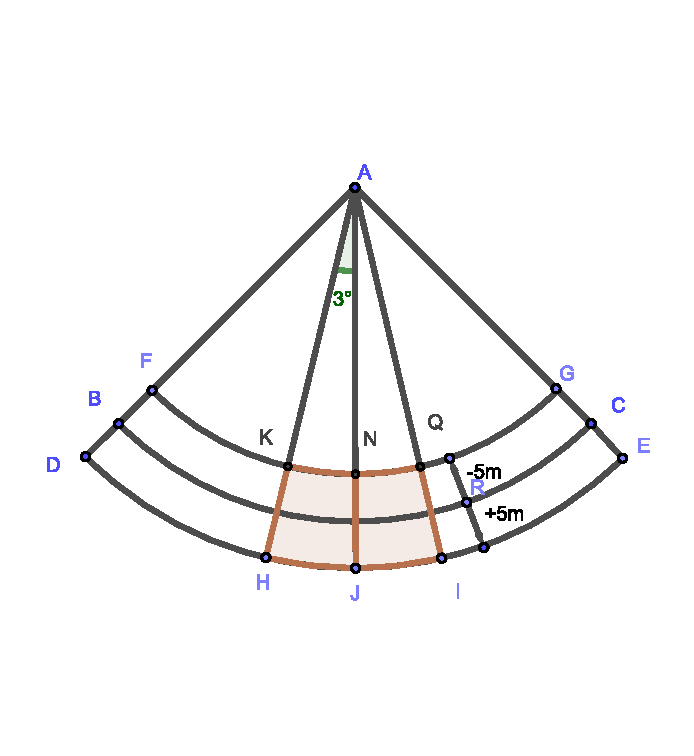
\includegraphics[width=0.45\linewidth]{pic/error area.eps}
  \caption{误差范围示意图}
  \end{figure}

模拟方式为在9个编号点中选取其中3个,两个点为发射点,一个点为接收点,给接收点设置一个随机扰动,得到一组模拟真实数据。计算接收点与发射源间的方向信息后,将其作为输入,用上文所建的模型进行求解后,得到一组求解数据。用模拟真实数据与求解数据进行比较,以此判断模型的准确性。

选取方案总共有$\begin{pmatrix} 3 \\ 9 \end{pmatrix}\times 3=252$种,将其全模拟并且在随机扰动十万次后,发现模拟真实数据与求解数据间的误差在小数点10位之后,考虑为机器误差。由于数据量过大,故不将具体数据放入正文及附录中,具体内容可见于支撑材料。

\subsubsection{发射源的选取}

共有四类发射源的选取方式,分别与原点的夹角为$\pm 40^{\circ}$,$\pm 80^{\circ}$,$\pm 120^{\circ}$,$\pm 160^{\circ}$。

不断扩大误差范围,直至扩大到误差为30\%(即极径误差限扩大为$\pm 15m$,幅角误差限扩大为$\pm 3^{\circ}$时,出现“报错现象”。“报错现象”的定义为模拟真实位置与求解位置之间的距离超过机器误差eps(根据经验,约为$10^{-8}$)。

在上部分的模拟中,这四类情况我们均有涉及,现为扩大数据量,增加实验可信度,每轮模拟次数调整为10000000次。其中,发射源的圆心角为$40^{\circ}$时,报错概率较小,约为其他几类情况报错概率的$\frac{1}{2}$。

运行三轮的数据基本保持稳定,具体结果如下图所示:

\begin{figure}[htbp]
  \centering
  \includegraphics[width=0.75\linewidth]{pic/Rplot01.jpeg}
  \caption{不同发射源圆心角的报错频次图}
  \end{figure}




故在进行发射源的选取时,可以尽可能多考虑圆心角为$40^{\circ}$的两个无人机作为发射源。


\subsection{问题二模型的建立与求解}

\subsubsection{角度区间定位模型}

b.当将获得的方向信息对应在相应的角度区间上时,我们可以判断未知发射源无人机的可能编号。编号的可能性一般有两种且关于FY01号无人机的位置对称







\end{document}